\documentclass[10pt,a4paper]{article}

\usepackage[utf8]{inputenc}
\usepackage[T1]{fontenc}
\usepackage[svgnames]{xcolor} % Required to specify font color
%\usepackage{mathpazo} %fancy font used by Anthony
\usepackage{floatrow}
\usepackage{geometry}%réglages mise en page
\geometry{%
a4paper, % note : l'option a4paper tuait la marge supérieure.
body={170mm,250mm}, %
left=25mm,top=25mm,right=25mm, %
headheight=21mm,headsep=7mm,
marginparsep=4mm,
marginparwidth=20mm, %
footnotesep=50mm
}

\usepackage{graphicx}
\usepackage{float}
\usepackage{color}
\usepackage{amssymb}

\usepackage{array}
\usepackage{hyperref}
\usepackage{lscape}

%%% Pour colorier le code source C++/matlab
\usepackage{listings}
\usepackage{xcolor}
\usepackage[colorinlistoftodos]{todonotes}

\definecolor{colKeys}{rgb}{0,0,1}  % couleurs des mots-clés propres au language
\definecolor{colIdentifier}{rgb}{0,0,0}  % couleurs des mots à identifier
\definecolor{colComments}{rgb}{0,0.6,0}  % couleurs des commentaires
\definecolor{colString}{rgb}{0.6,0.1,0.1}

\lstset{language=c++}
\lstset{commentstyle=\color{colComments}\textit, %
basicstyle=\ttfamily\small, %
identifierstyle=\color{colIdentifier}, %
keywordstyle=\color{colKeys}, %
stringstyle=\color{colString}, %
commentstyle=\color{colComments}, %
columns=flexible, %
tabsize=2, %
extendedchars=true, %
showspaces=false, %
showstringspaces=false, %
numbers=left, %
numberstyle=\tiny, %
breaklines=true, %
breakautoindent=true, %
captionpos=b,%
}

\title{INFO-F-412 Formal Verification of Computer Systems\\The GOAT-IE\\ \large{The Gate Opener Action by Ticket -- Improved Edition}}
\author{Quentin Delhaye}

%%%%%%%%%%%%%%%%%%%%%%%%%%%%%%%%%%%%%%%%%%%%%%%%%%%%%%%%%%%%%%%%%%%%%%%%%%%%%%%%%%%

\begin{document} 
\maketitle

%%%%%%%%%%%
\section{Introduction}
%%%%%%%%%%%
This project directly follows the Embedded Systems Design project.
In that project, entitled "\textit{The GOAT}", we modelised a sas with two doors.
When the sas was not occupied, the first door was open for anyone to enter.
Uppon user entering, the first door would close and a timer would begin.
In the given time, the user could present his card to be processed by the sas, or simply leave the sas by the first door.
If the card was accepted, the second door would open for the user to leave.
While doing all those actions, the timer clock would progress, and when reaching its limit, broadcast a signal to the user asking him to leave the sas by the first door, so that he would not stay in there forever.

In the present project, we want to improve the behavior of the sas by adding a queue for him to handle, in order to guarentee a fair sequence of users entering the sas.

%%%%%%%%%%%
\section{Improvement to the models}
%%%%%%%%%%%
The larger part of the models where not modified.
As we want to control the flow of users entering the sas, the new part involves the transition to and from \texttt{User.in\_sas}.

\begin{lstlisting}[caption=Global system declarations., label=lst:globalDecl]
chan infra1, infra2, cardIn, eject
chan req;//Request channel
clock timeInSas;
const int SAS_TIMER = 10;
const int N_USERS = 2;
int reqID;
int turn;//The ID of the user whose it's turn.
int gateConf = 1;//Binary: g2g1 => 01 = gate 2 closed && gate 1 open, 00 both closed, 10 = gate 2 open && gate 1 closed.
int userCard;
\end{lstlisting}

\subsection{User}
In the user model, we add a new state \texttt{want\_in} that will be a pool in which the user goes if he, as the state name suggests, wants in.
The transition from \texttt{before\_sas} to \texttt{want\_in} triggers a signal \texttt{req} that will be followed in the sas model.

The second and last modification in this system is the new guard on the transition \texttt{want\_in} to \texttt{in\_sas}. Indeed, the user now has to wait for his turn, represented by the variable \texttt{turn} being set to his id.

The figure~\ref{fig:userModel} and listing~\ref{lst:userDecl} present this updated model. It is also to be noted that all users have a copy of the same model.

\begin{figure}[!h]
	\centering
    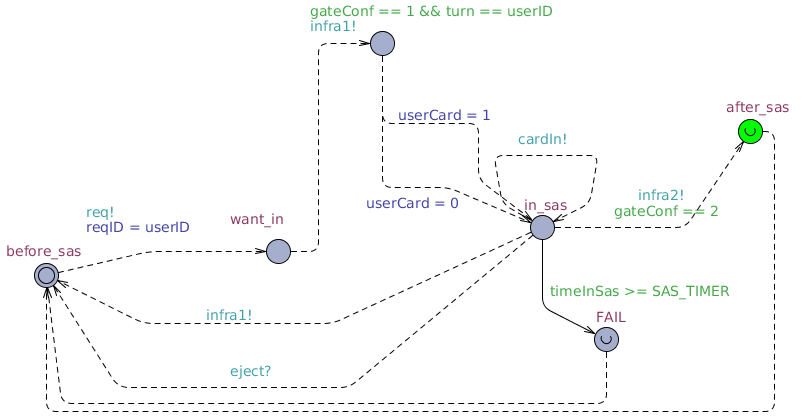
\includegraphics[width=\textwidth]{userModel}
    \caption{New user model with request token.}
    \label{fig:userModel}
\end{figure}

\begin{lstlisting}[caption=Declarations of user model., label=lst:userDecl]
clock x;
const int userID = 1;
\end{lstlisting}

\subsection{Sas}
The first modification is the addition of new self-transitions on \texttt{idle} and \texttt{handling\_user} states for the reception of the signal \texttt{req}.
When receiving the signal, the sas receives the id the corresponding user and adds it to the queue using the \texttt{addInQueue(int)} function.

When the user enters the sas, the sas model shifts the queue using \texttt{shiftQueue()} so that the next user in line is ready to enter as soon as the sas is available.

The figure~\ref{fig:sasModel} and listing~\ref{lst:sasDecl} present this updated model.

\begin{figure}[!h]
	\centering
    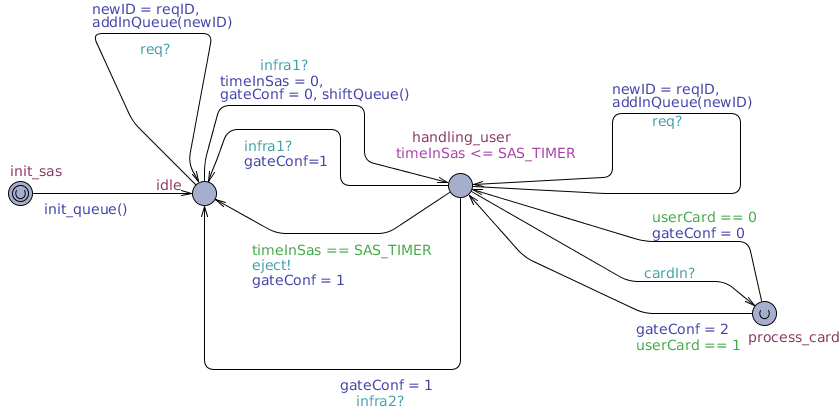
\includegraphics[width=\textwidth]{sasModel}
    \caption{New sas model with queue handling.}
    \label{fig:sasModel}
\end{figure}


%%%%%%%%%%%
\section{Winning conditions}
%%%%%%%%%%%
Some winning condition have already been discussed in the Embedded Systems Design report.
For the new properties of the system, we may add the following expressions using \textsc{CTL}:
\begin{itemize}
	\item $\forall$\verb|[] (User.want_in |$\rightarrow \forall$ \verb|<> User.in_sas)| ~\\
		If the user want to enter the sas, he will enter the sas (liveness).
	\item $\forall$\verb|[] (User.before_sas |$\rightarrow \exists$ \verb|<> User.want_in| ~\\
		If the user is in idle mode, he will be able to request entering inside the sas (non-blocking).
	\item $\forall$\verb|[] not(User.in_sas and User2.in_sas)| ~\\
		Two users can not be in the sas at the same time (safety)\footnote{For the sake of completion, as this property was already presented in the linked project.}.
\end{itemize}

%%%%%%%%%%%
\section{Conclusion}
%%%%%%%%%%%
This project extends the one for Emebdded Systems Design by repairing one of its fault that was one user could monopolize the sas by leaving and entering it directly without giving other user a fair chance to access the said sas.
In a sense, we did enforce some sort of strict sequencing, but only to ensure a certain degree of fairness in the system. 
It is simply the modelisation of a real-life problem: poeple enter a queue to access a ressource that can only be used by one person for a certain amount of time.

If we want to take this project even one step further, we could make the sas two-way, instead of one.
In this improvement, both doors could be closed in idle mode and users could request its accessed from the first or the second door.
The modelisation would not differ that much, since we can use the same queue to store the requests, and the distribution mechanism of tokens would be sensibly the same.

\newpage
\appendix
%%%%%%%%%%%
\section{Sas declarations}
\begin{lstlisting}[caption=Sas model declarations., label=lst:sasDecl]
clock x;

int queue[N_USERS];
int newID;//Requester's ID

void init_queue()
{	
	int i;
	for(i = 0;i<N_USERS;++i) {
		queue[i] = 0;
	}
}

//Add a new id at the end of the queue
void addInQueue(int id) 
{
	int i;
	int set = 0;
	for(i=0;i<N_USERS && set==0;++i) {
		if(queue[i] == 0) {
			queue[i] = id;
			set = 1;
		}
	}
	turn = queue[0];//Update if necessary
}

//Shift each user one place forward in the queue
void shiftQueue()
{
	int i;
	for(i=0;i<N_USERS-1;++i) {
		queue[i] = queue[i+1];
	}
	queue[N_USERS-1] = 0;//Last place in the queue is available.
	turn = queue[0];//Update if necessary
}
\end{lstlisting}


\end{document}
